% Appendix
%
%	Experimental Set-up
%	Model Equations

\appendix\addtocontents{toc}{\protect\newpage}
\glsresetall
\chapter{Estimation of the amount of data}

Presently the \gls{LHC} is working with an interval of 50~ns between \glspl{bunch}. This correspond to a bunch every 20 \glspl{bucket}. But the \gls{OP} is planning to move to 25ns \glspl{bunch} spacing. This would mean 5 \glspl{bucket} between \glspl{bunch}. With the \gls{rffreq} we can compute the number of acquisitions per seconds.

$${\rm for~}50{\rm ~ns}~: \frac{400.789*10^{6}}{20} = 20\;039\;450 \leq 2^{25}$$

$${\rm for~}25{\rm ~ns}~: \frac{400.789*10^{6}}{10} = 40\;078\;900 \leq 2^{26}$$ 

This represent the amount of data for one pickup (\gls{BPM}), in the case of \gls{ADT} we have two of them per beam and per plane. The \gls{LHC} has two rings, for each ring there are two transversal planes, and there are two pickups per plane. Therefore we have to multiply this value by eight.

$${\rm for~}50{\rm ~ns}~: 2^{25} * 8 = 2^{28}$$

$${\rm for~}25{\rm ~ns}~: 2^{26} * 8 = 2^{29}$$

As \glspl{FFT} on \glspl{GPU} start to be be faster than \glspl{CPU} around $2^{15}$ acquisitions it seems interesting to study this kind of system to compute the \gls{tune}.

\chapter{Measurement with the ADT}

In order to check the feasibility of the system and to have a good prototype the first test will be to excite some of the \glspl{bunch} and acquire the \gls{tune} using the \gls{ADT} during the end of 2012 run\cite{Valuch12}.

A piece of software has been developed that will receive the bunch by bunch acquisition and run various algorithm on the data using the \gls{CPU} and the \gls{FFTW} library in the \gls{CERN} infrastructure using \gls{CO} group control system and the \gls{OP} group infrastructure.

\section{Experimental Set-up}

This is a basic description of the setup used during the \gls{MD} of 2012 during witch some data acquisition was made in the \gls{LHC}. The low level analog part of the system is the same as the system that will be used in the future system, but some parts described were not present at the moment of the data acquisitions.

\subsection{Hardware}

The experimental set up is not presently able to acquire more than a certain number of bunches due to memory limitation of 16k and limitations in interrupt frequency. Therefore, during the \glspl{MD}, only 6 bunches were acquired per beam and per plane.

\subsection{Software}

The software used during data acquisition was only able to get the data from the card and copy it on a disk that was available on the \gls{CERN} \gls{NFS}. The software was able to compute the \gls{FFT} but only using \gls{FFTW} and no \gls{GPU}.

\chapter{Machine development sessions}

Using the \gls{ADT} \glspl{BPM} we acquired data in the machine during 3 independent \glspl{MD}. Most of the data was taken in parallel during normal LHC operation or during \gls{ADT} dedicated \gls{MD} time.

\section{First session}

Night session of the 11 October 2012.

This was the first session and the software still had some issues. We experienced some difficulties in injecting in the \gls{LHC} that were not really related to us.

Overall we got some nice result and that was very encouraging for further test.

\begin{figure}[H]
\centering
\begin{subfigure}{.5\textwidth}
  \centering
  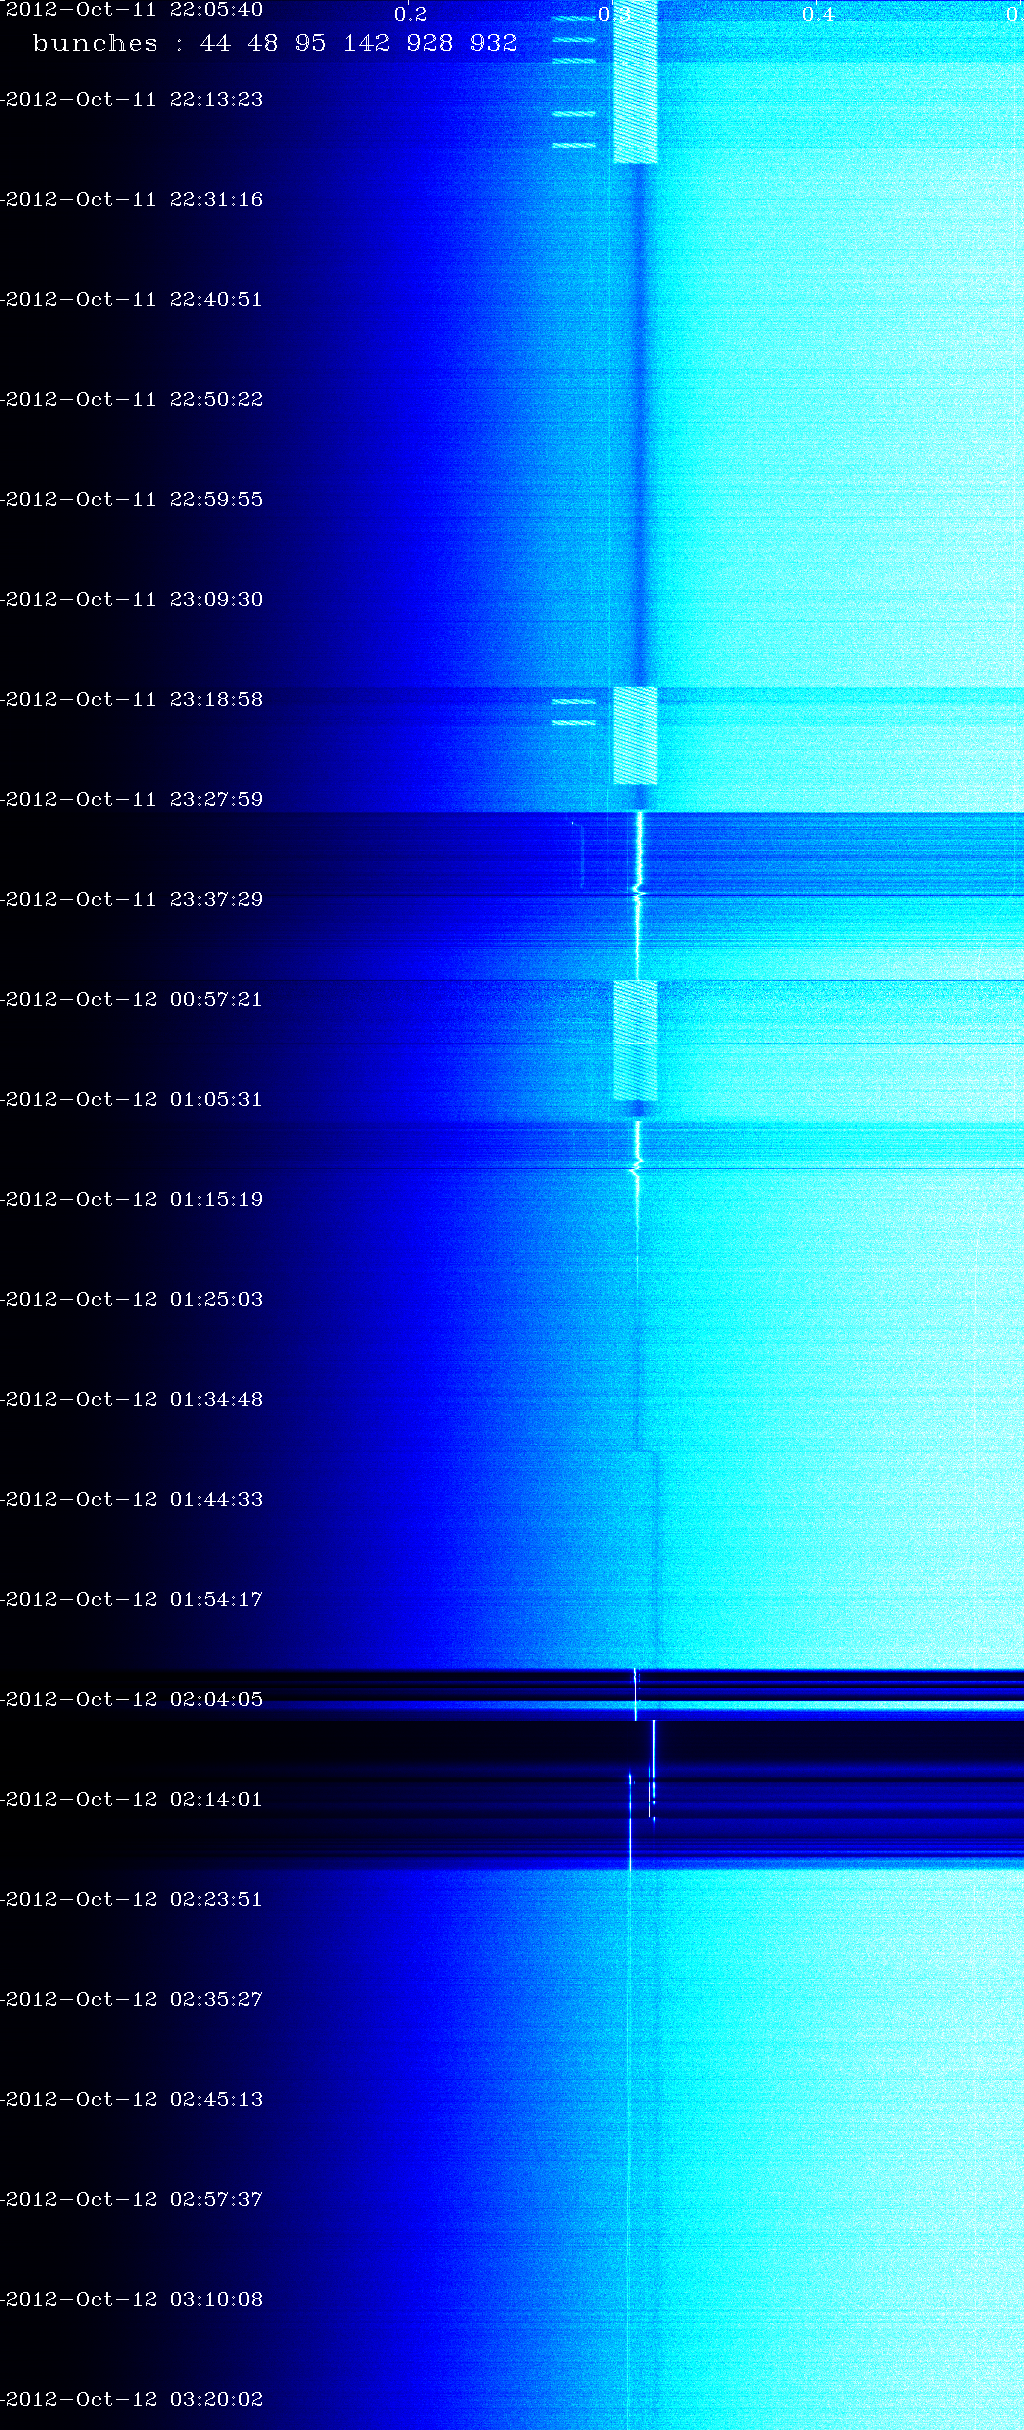
\includegraphics[width=.8\linewidth]{md-121011-vb2-bunches111111-16.png}
  \caption{Vertical beam 2}
\end{subfigure}%
\begin{subfigure}{.5\textwidth}
  \centering
  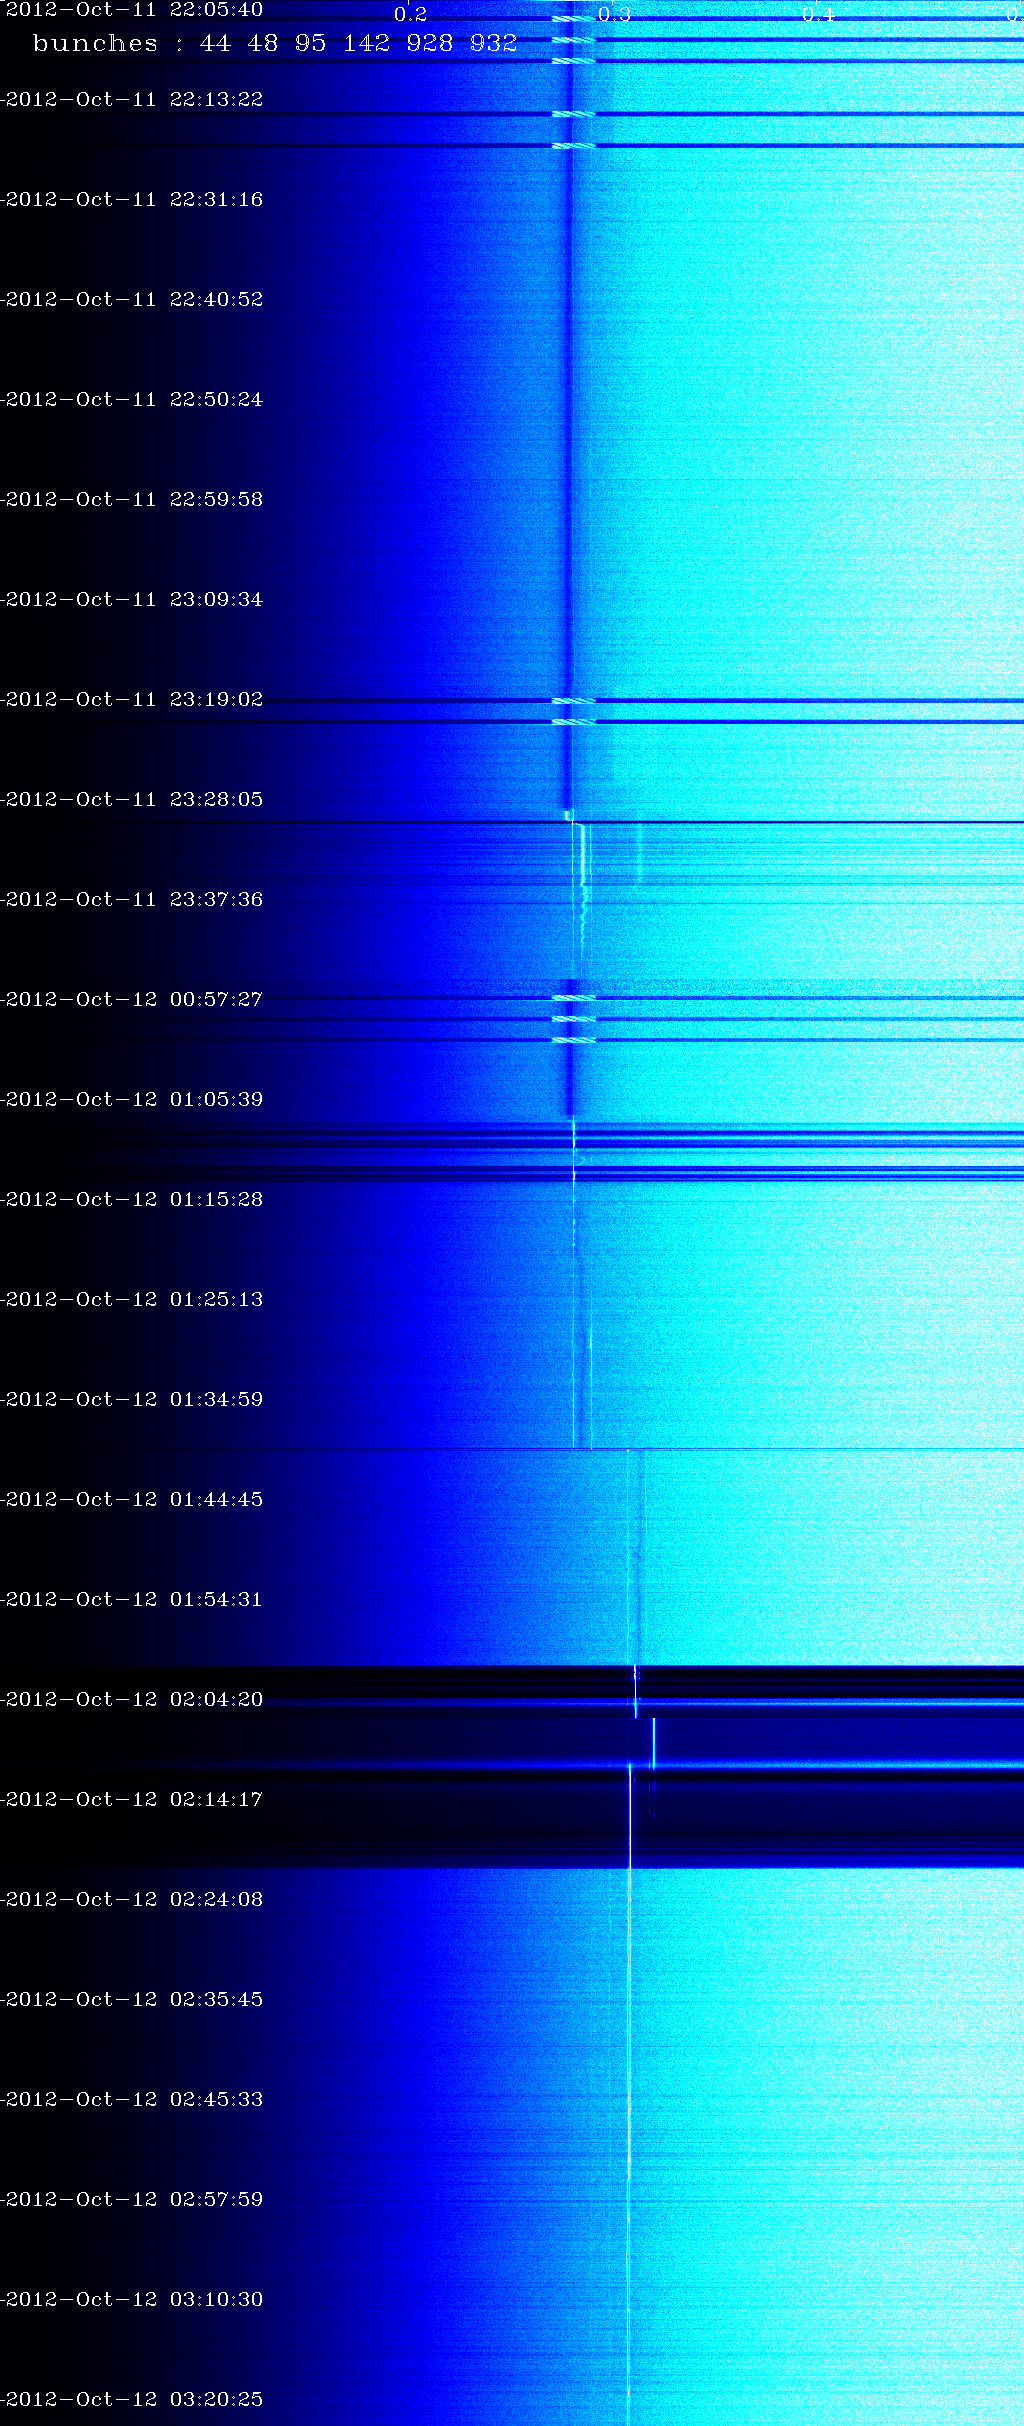
\includegraphics[width=.8\linewidth]{md-121011-hb2-bunches111111-16.png}
  \caption{Horizontal beam 2}
\end{subfigure}
\caption{Spectrograms of the full 11 of October 2012 session on Beam 2}
\end{figure}

\section{Second session}

Parasitic session of the 16 October 2012. 

The bugs were fixed and we could have a short acquisition session that happen in parallel with other operation.

This session allowed us to validate the acquisition software in normal operation and with the changes that where made in between the two \gls{MD}.

\begin{figure}[H]
\centering
\begin{subfigure}{.5\textwidth}
  \centering
  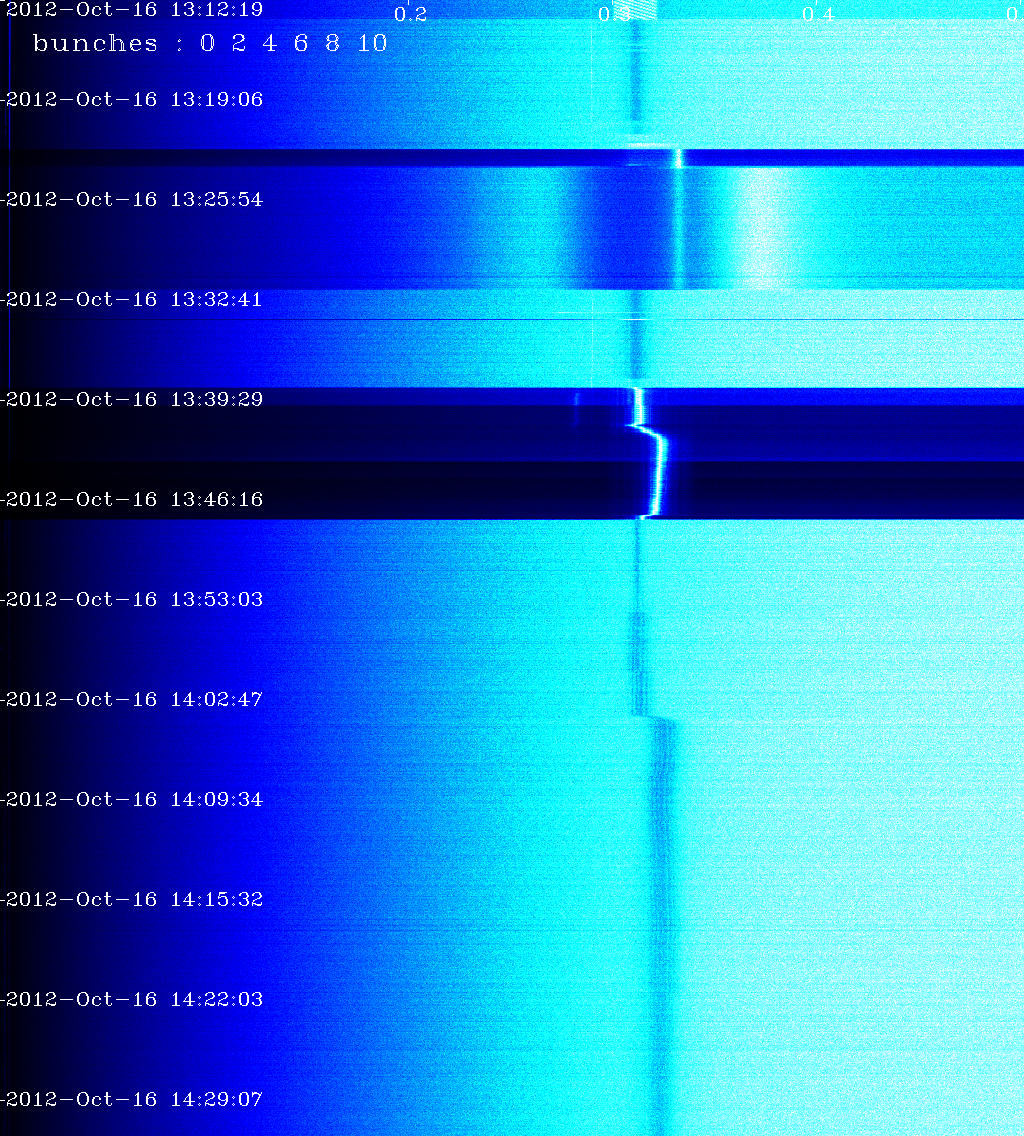
\includegraphics[width=.8\linewidth]{md-121016-vb1-bunches111111-16.png}
  \caption{Vertical beam 1}
\end{subfigure}%
\begin{subfigure}{.5\textwidth}
  \centering
  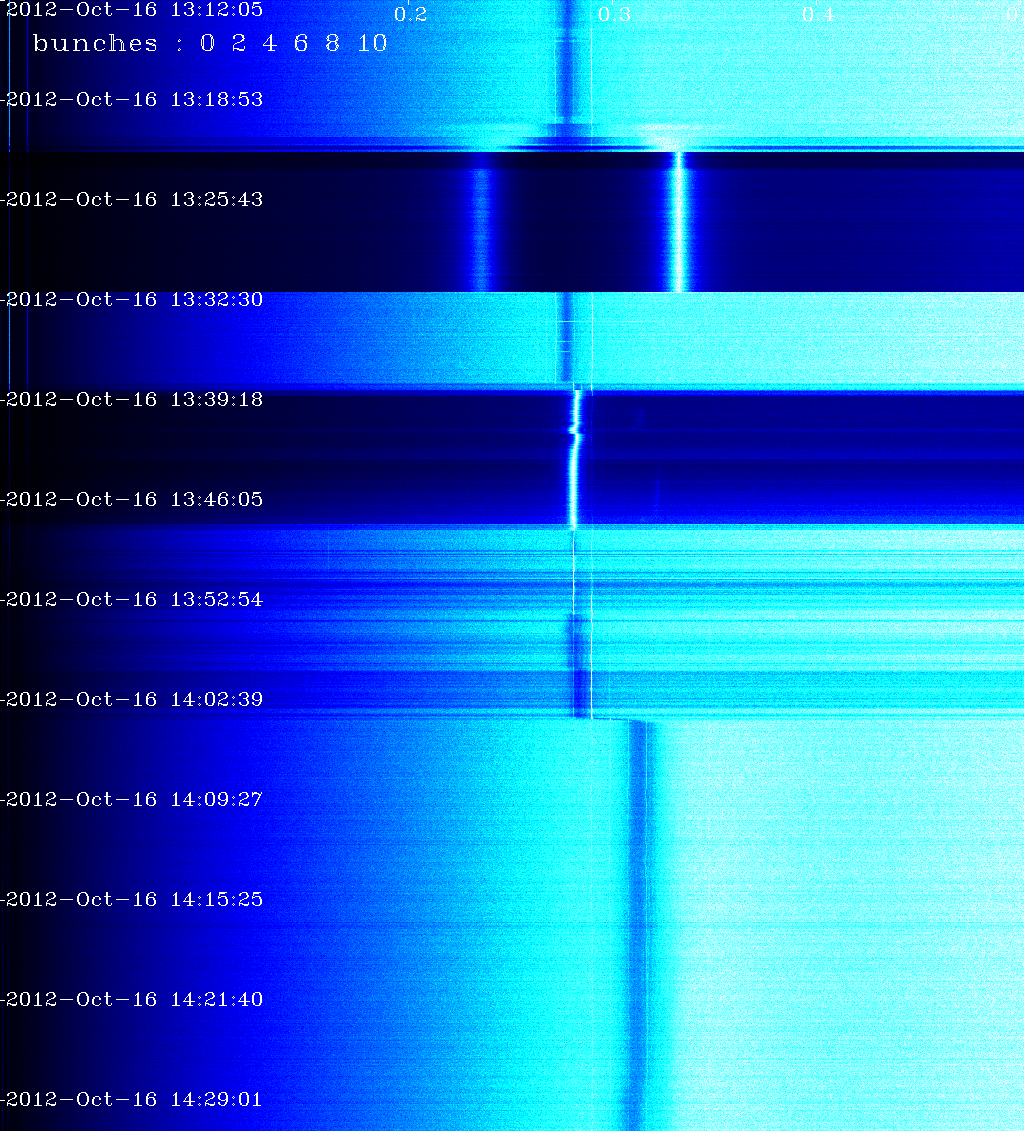
\includegraphics[width=.8\linewidth]{md-121016-hb1-bunches111111-16.png}
  \caption{Horizontal beam 1}
\end{subfigure}
\caption{Spectrograms of the full 16 of October 2012 session on Beam 1}
\end{figure}

\section{Third session}

Ramp acquisition of the 14 November 2012. 

During this afternoon we had some machine time to acquire the tune with the acquisition software on low gain bunches during ramp and collision.

The software worked well but the noise at the end of the ramp was too big and the tune was not obviously visible.

\begin{figure}[H]
\centering
\caption{Spectrogram of the full 14 of November 2012 session on horizontal beam 1}
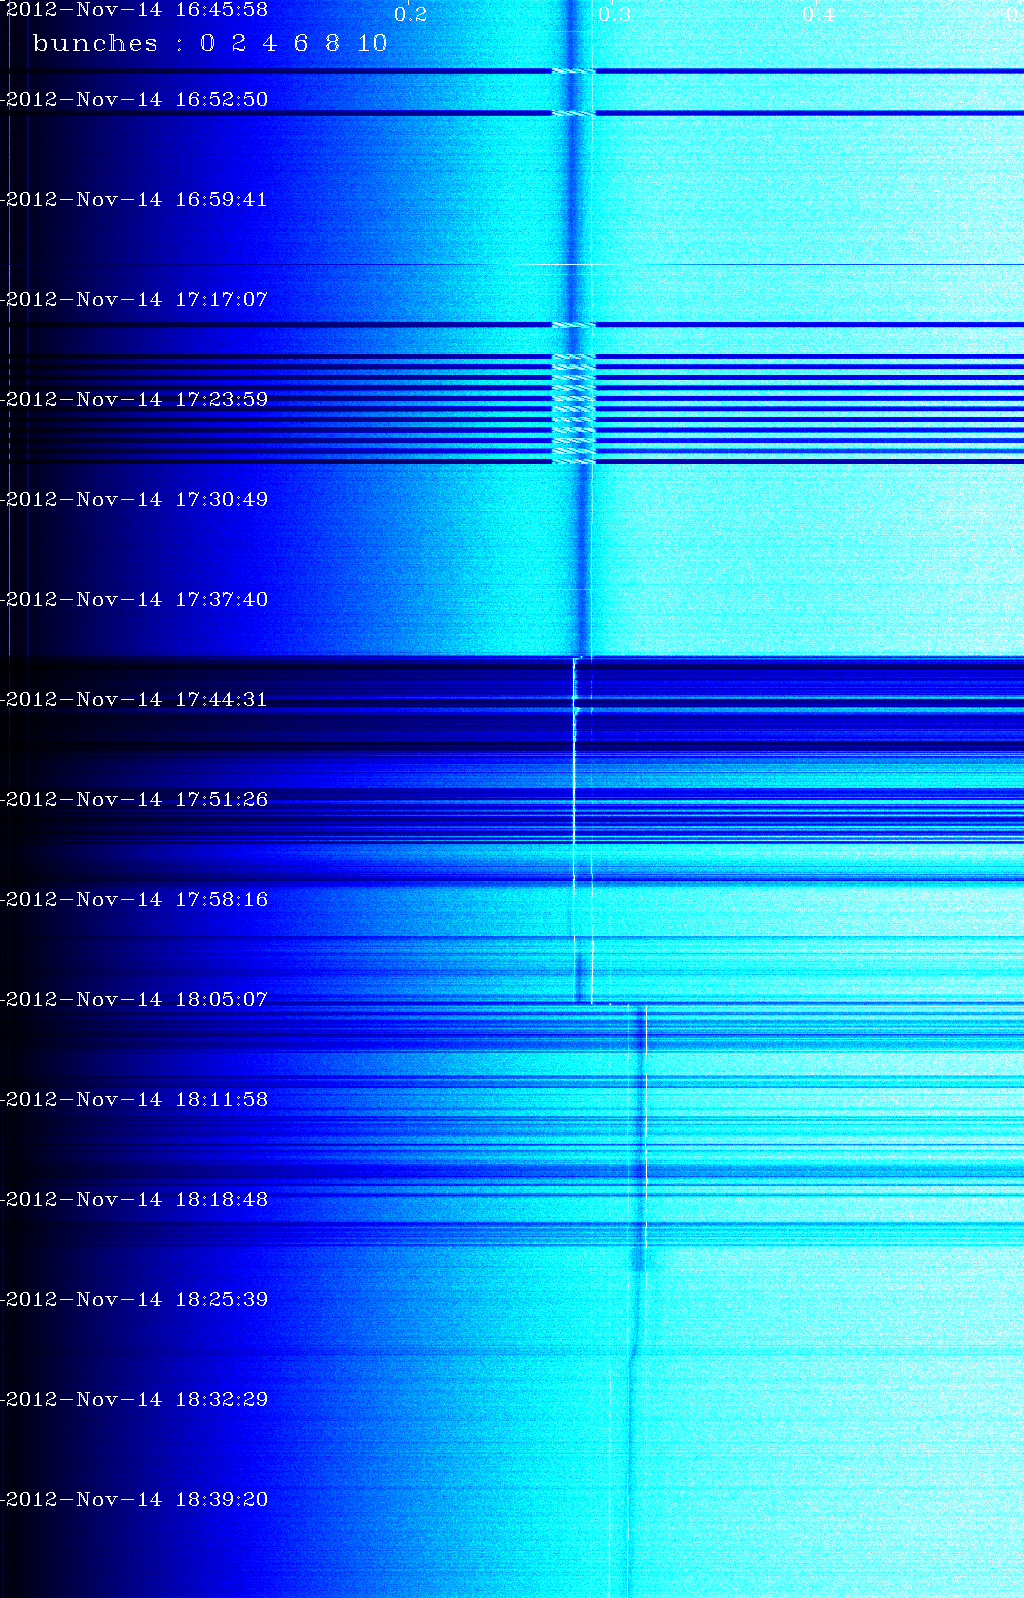
\includegraphics[scale=0.3]{md-121114-hb1-bunches111111-16.png}
\end{figure}

\chapter{Source code}

The source code is available online for the data analysis software under GIT and inside the \gls{CERN} infrastructure for the \gls{FESA} classes under CVS. Code published by \gls{CERN} is by default under \gls{GPL} v3.

\section{FESA ADTDSPU}

The source files for the \gls{ADTDSPU} \gls{FESA} class is available on \gls{CERN} central \gls{CVS} servers (only from inside CERN network) at~: \url{http://isscvs.cern.ch/cgi-bin/viewcvs-all.cgi/ALLADTDSPU/v210/?root=FESA-equipment}.

\section{FESA Tune Acquisition}

The source files for the tune acquisition software is also available on \gls{CERN} central \gls{CVS} servers (only from inside CERN network) at~: \url{http://isscvs.cern.ch/cgi-bin/viewcvs-all.cgi/ALLADTTuneMeas/v0/?root=FESA-equipment}.

\section{Data analysis}

The source files for the data analysis software are available on GitHub at~: \url{https://github.com/anirul/TM\_LHC\_tune} and is under BSD type license.
